\documentclass[12pt]{article}
\usepackage[utf8]{inputenc}
\usepackage{amsmath}
\usepackage[T1]{fontenc}

\title{ECE 3413 Lab 10\\*Closed Loop Gain Determination using Root Locus}
\author{Leomar Dur\'an}
\date{${23}^{\text{th}}$ April 2023}

\usepackage{pdflscape}

\usepackage[natbib,style=apa6]{biblatex}
\addbibresource{main.bib}
\defbibheading{bibliography}[\refname]{%
  \section*{\centering #1}%
}%

\usepackage{hyperref}

\usepackage{cancel}
\usepackage[per-mode=symbol]{siunitx}
\newcommand*\siexpr[2][]{\SI[parse-numbers=false,#1]{#2}}%
\DeclareSIUnit\bel{B}
\DeclareSIUnit\byte{Byte}

\usepackage{xfrac}
\usepackage{amssymb}
\newcommand*\transpose{\mathsf{T}}

\usepackage{mathtools}%
\DeclarePairedDelimiter\brao()%
\DeclarePairedDelimiter\brac[]%
\DeclarePairedDelimiter\braco[)%
\DeclarePairedDelimiter\braoo][%
\DeclarePairedDelimiter\Brac\{\}%
\DeclarePairedDelimiter\abs||
\DeclarePairedDelimiter\norm\lVert\rVert%
\DeclarePairedDelimiter\piecefn\{.
\DeclarePairedDelimiter\evalat.|

\usepackage{lib/nonfloatenvirons}
\usepackage{booktabs}
\newcommand\ra[1]{\renewcommand*\arraystretch{#1}}
\ra{1.25}

\usepackage{minted}
\newcommand\matlab{matlab}

\usepackage{adjustbox}
\newcommand{\setprime}[2][1]{%
    {#2}^{%
        \raisebox{1pt}{%
            \scalebox{0.5}{%
                \itshape\sffamily\uppercase%
                \expandafter{%
                    \romannumeral#1%
                }%
            }%
        }
    }%
}%
\newcommand*\mcadj[7]%
% {#columns}{col spec}{rotation}{adjust spec}
% {before rotated text}{rotated text}{after rotated text}
{%
    \multicolumn{#1}{#2}{%
        \rlap{%
            #5\adjustbox{rotate=#3,#4}{#6}~#7%
        }%
    }%
}

\usepackage{pdfpages}
\usepackage{standalone}
\usepackage{matlab}

\usepackage[skip=\baselineskip,indent=0pt]{parskip}
\setlength\parindent{0pt}

\usepackage[shortlabels]{enumitem}

\def\hr{{\par\noindent\rule{\textwidth}{0.4pt}}}

\begin{document}

\maketitle
\newpage

\section{Introduction}\label{sec:intro}

\subsection{The setup}\label{ssc:the setup}

For this lab,
we will need to install the System Identification Toolbox add-on.

Before starting the installation,
be warned that the installation will require escalation to Administrator privileges.
One will also need to agree to ``The MathWorks, Inc. Software License Agreement''
as the System Identification Toolbox add-on as created by MathWorks%
{} (as of this writing).
After the installation, \textsc{Matlab} will restart,
so save all previous work first.

Additionally,
this add-on has no additional dependencies.
The download is $\SI{61}{\mega\byte}$ and the installation is $\SI{160}{\mega\byte}$.

\begin{enumerate}
    \item
        Once ready,
        open the Home tab,
        and find the Add-Ons menu in the \textsc{environment} section
        as shown in Fig.~\ref{fig:finding addons},
        and click the Get Add-Ons button highlighted.

        \begin{figure}
            \centering
            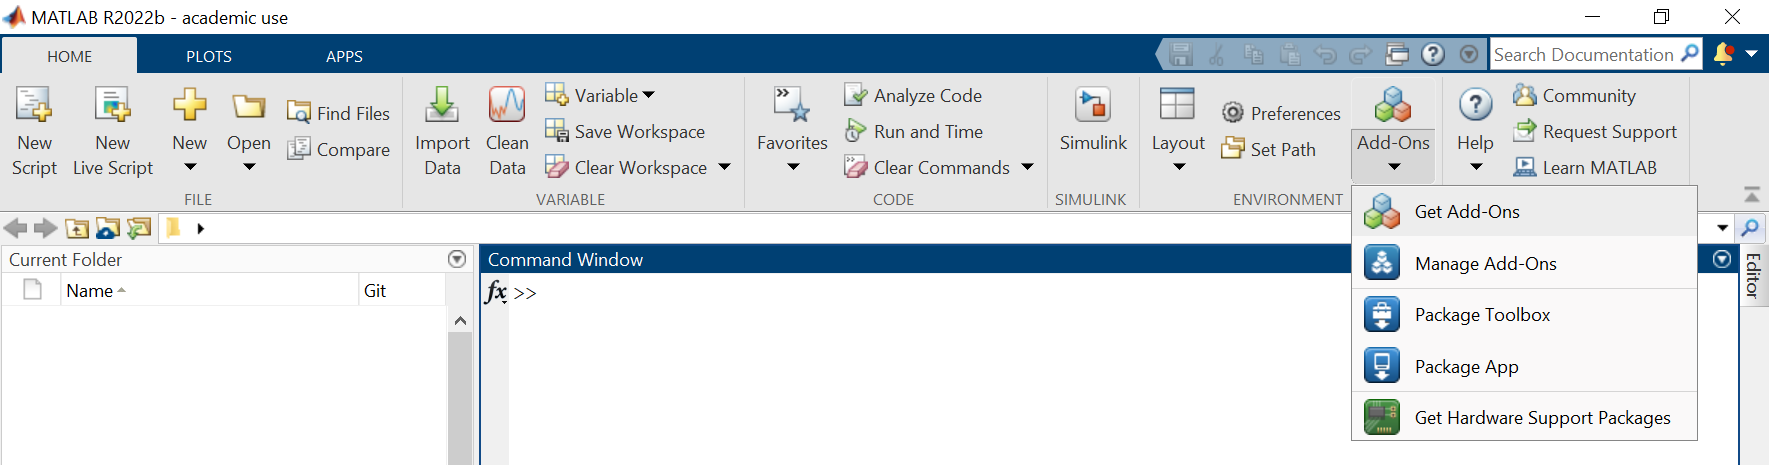
\includegraphics[width=\linewidth]{img/intro_010_finding_addons.png}
            \caption{Finding the Add-Ons menu.}
            \label{fig:finding addons}
        \end{figure}

    \item
        In the search bar of the ``Add-On Explorer'' dialog opened,
        search for ``Simulation Control Design''.
        It is the first hit in the results listed in Fig.~\ref{fig:searching System Identification Toolbox}.

        \begin{figure}
            \centering
            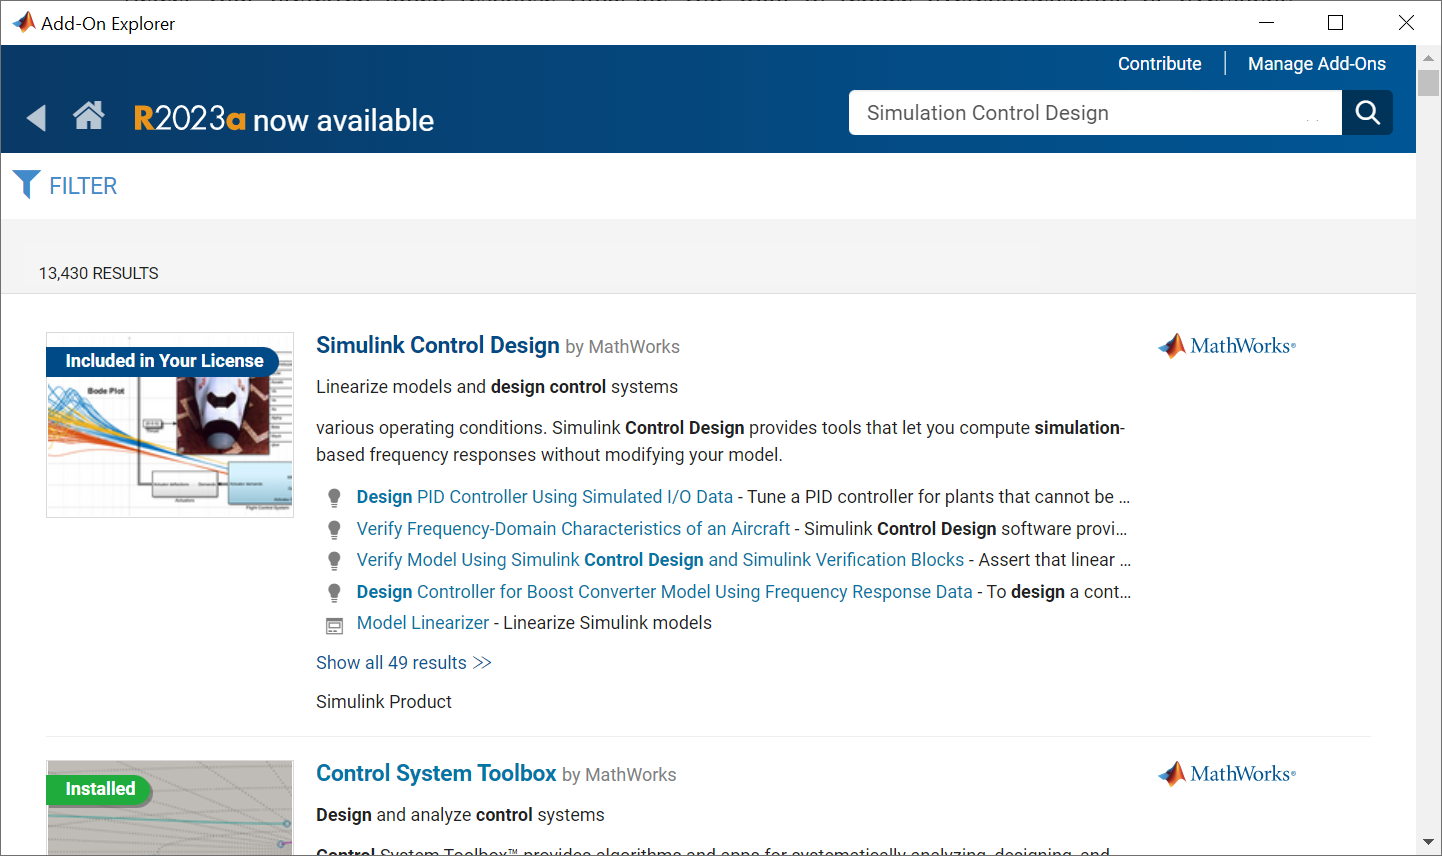
\includegraphics[width=\linewidth]{img/intro_020_searching_simulink_control_design.png}
            \caption{The ``Add-On Explorer'' dialog with ``Simulation Control Design'' hovered in navy blue text.}
            \label{fig:searching System Identification Toolbox}
        \end{figure}

        The Simulation Control Design add-on should be labeled
        with the navy blue ``Included In Your License'' label.
        However,
        if it was already installed,
        then you will see the green ``Installed'' label%
        {} seen in Fig.~\ref{fig:searching ìnstalled System Identification Toolbox},
        in which case,
        no further action is needed
        and you may proceed to Subsection~\ref{ssc:background} \nameref{ssc:background}.

        \begin{figure}
            \centering
            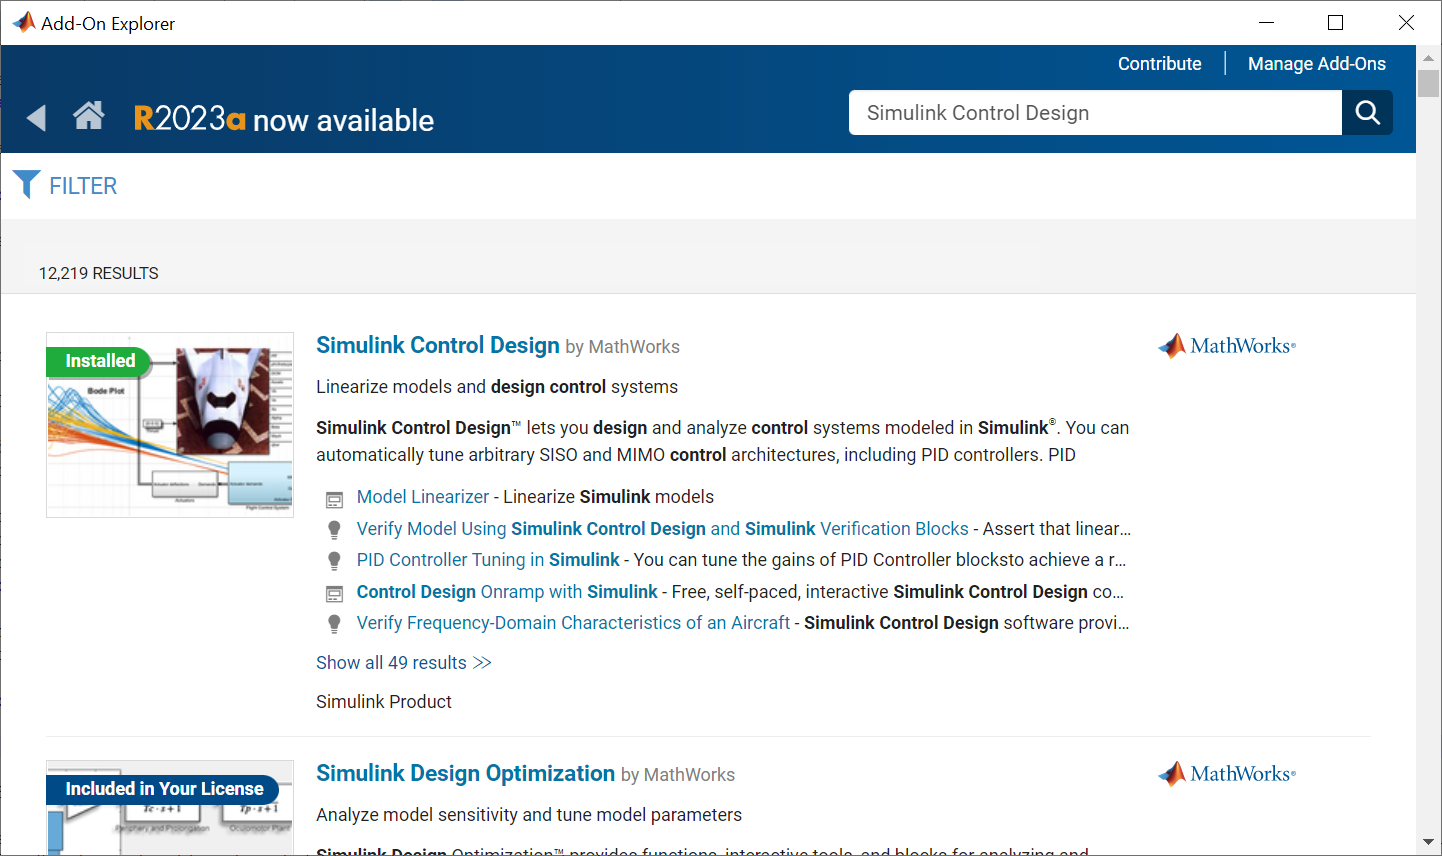
\includegraphics[width=\linewidth]{img/intro_050_searching_installed_simulink_control_design.png}
            \caption{The Simulation Control Design add-on already installed in the ``Add-On Explorer'' dialog.}
            \label{fig:searching ìnstalled System Identification Toolbox}
        \end{figure}

        However, if the label is different from either of these,
        please contact your administrator about licensing%
        {} before proceeding.

        Proceeding from Fig.~\ref{fig:searching System Identification Toolbox},
        click on the Simulation Control Design add-on to select it.
    \item
        To install,
        click on the Install button,
        which will highlight in light blue when hovered over like in Fig.~\ref{fig:selected System Identification Toolbox}.

        \begin{figure}
            \centering
            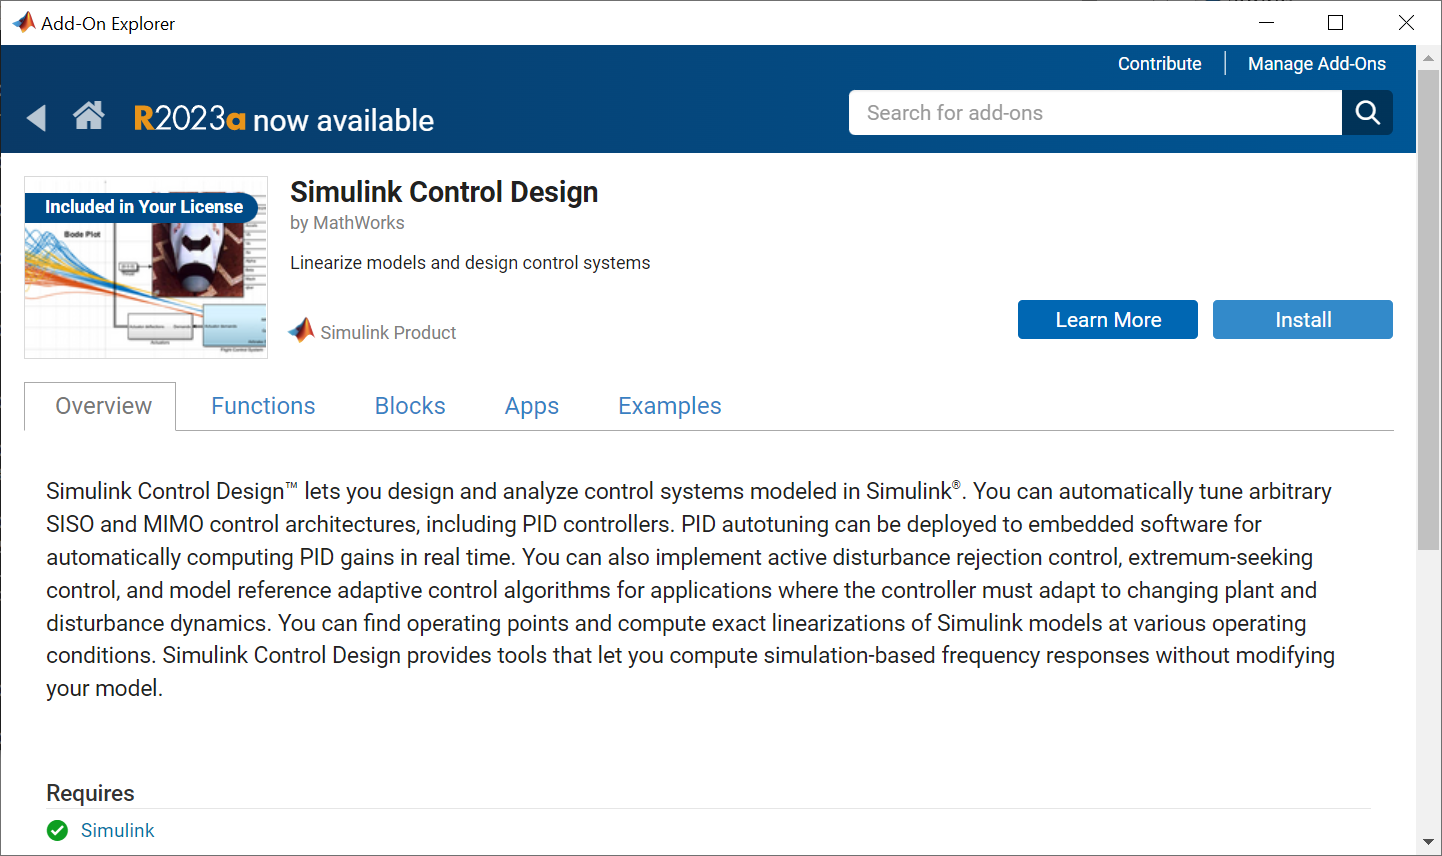
\includegraphics[width=\linewidth]{img/intro_030_selected_simulink_control_design.png}
            \caption{The Simulation Control Design add-on selected and ready for installation.}
            \label{fig:selected System Identification Toolbox}
        \end{figure}

        Follow the onscreen instructions,
        which will include escalation to Administrator privileges
        and agreeing to the ``The MathWorks, Inc. Software License Agreement''.

    \item
        \textsc{Matlab} will complete the installation process and restart,
        after which you will be greeted by the dialog in \ref{fig:System Identification Toolbox installation finished}.

        \begin{figure}
            \centering
            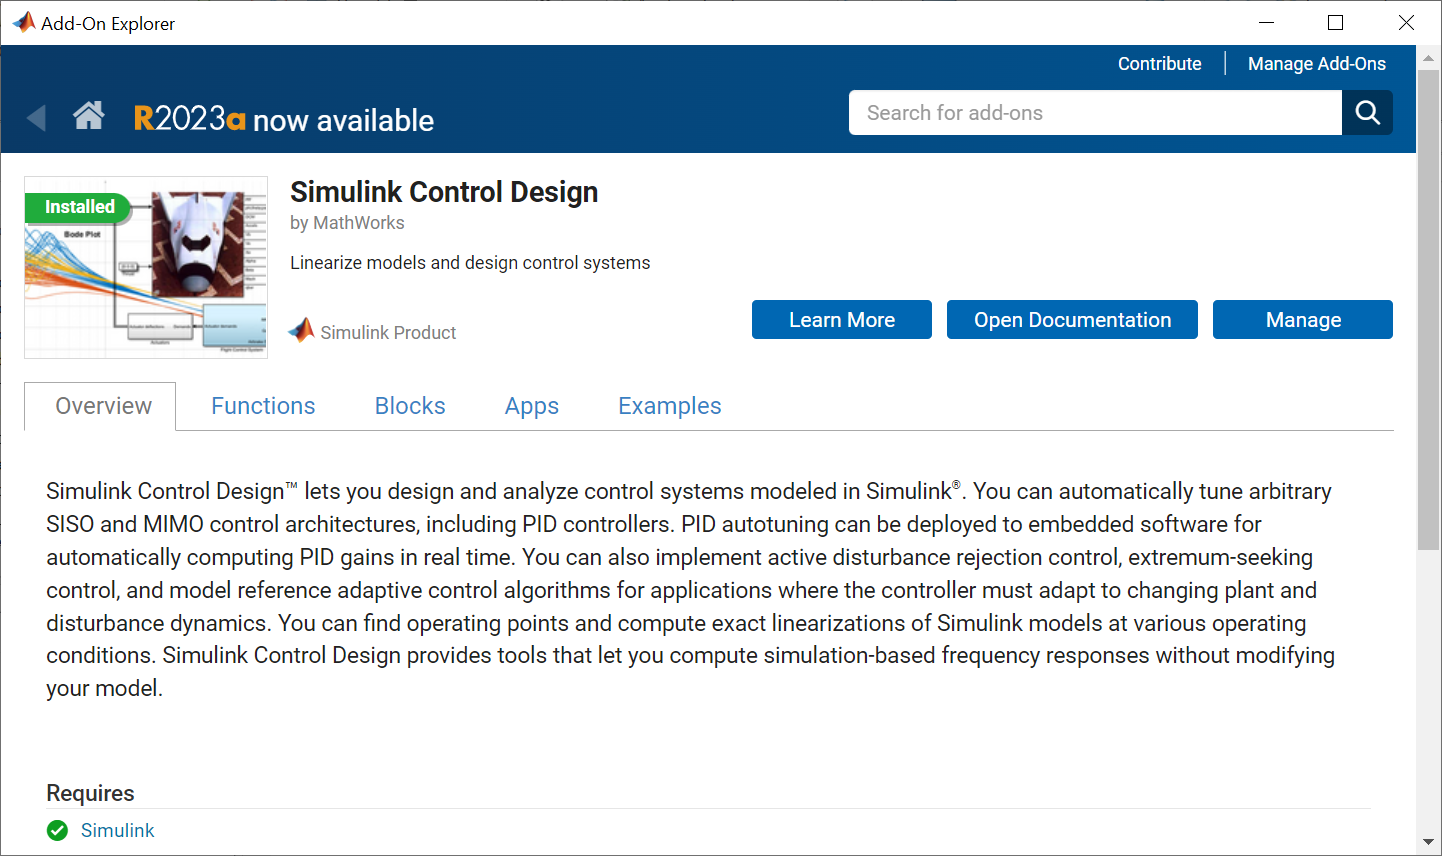
\includegraphics[width=\linewidth]{img/intro_040_installed_simulink_control_design.png}
            \caption{Dialog showing complete installation of the Simulation Control Design add-on.}
            \label{fig:System Identification Toolbox installation finished}
        \end{figure}
\end{enumerate}
\newpage

\subsection{Background information}\label{ssc:background}

The root locus technique may be used to find the optimal gains for a controller on a plant.

We will be applying this technique to a plant on noisy data.

\section{Procedure}\label{sec:Procedure}

\subsection{Task 00 -- Parameters}\label{ssc:parameters}

\begin{figure}
    \centering
    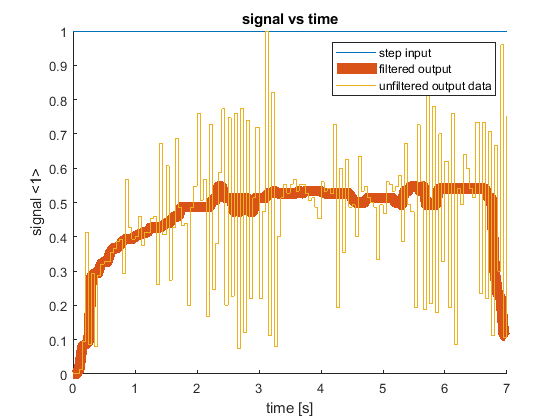
\includegraphics[width=\linewidth]{img/task01_viewing_data.png}
    \caption{Comparing the step input, raw output data and filtered output data.}
    \label{fig:viewing data}
\end{figure}

We start by loading the noisy data. From this data, we can reconstruct a step response triggered on $t = 0$, as well as apply a median filter to the data to create a smoother signal with similar rise and settling time characteristics.

To find the rise and settling time characteristics, we have
to smoothen the curve in the first place.  In light of this, a median
filter with 19o seems to smoothen out the function satisfactorily by
inspection
as can be seen in Fig.~\ref{fig:viewing data}.

This data parameterizes the transfer functions which we will estimate. The script for this parameterization is available in \nameref{app} subsection~\ref{sap:initial params}

% ident

Next we use the Matlab \mintinline\matlab{ident} function to call up the System Identification Toolkit.


\section{Results}

\subsection{Task 01 -- Varying the proportional terms}
\begin{figure}
    \centering
    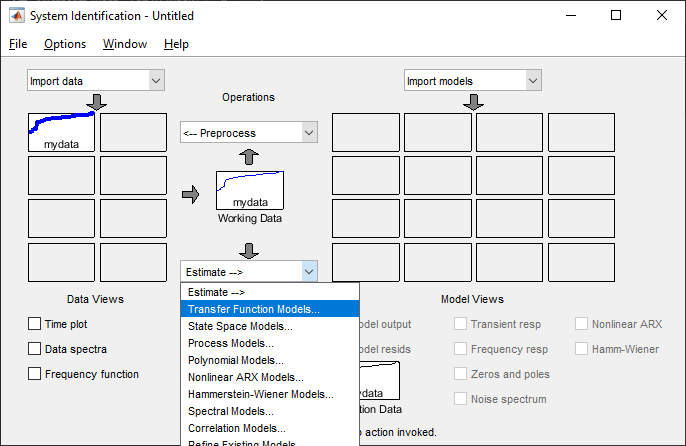
\includegraphics[width=\linewidth]{img/task03_030_modeling_tf.png}
    \caption{All transfer functions estimated in the System Identification Toolkit.}
    \label{fig:task 03-07 ident}
\end{figure}

\begin{landscape}
\begin{figure}
    \centering
    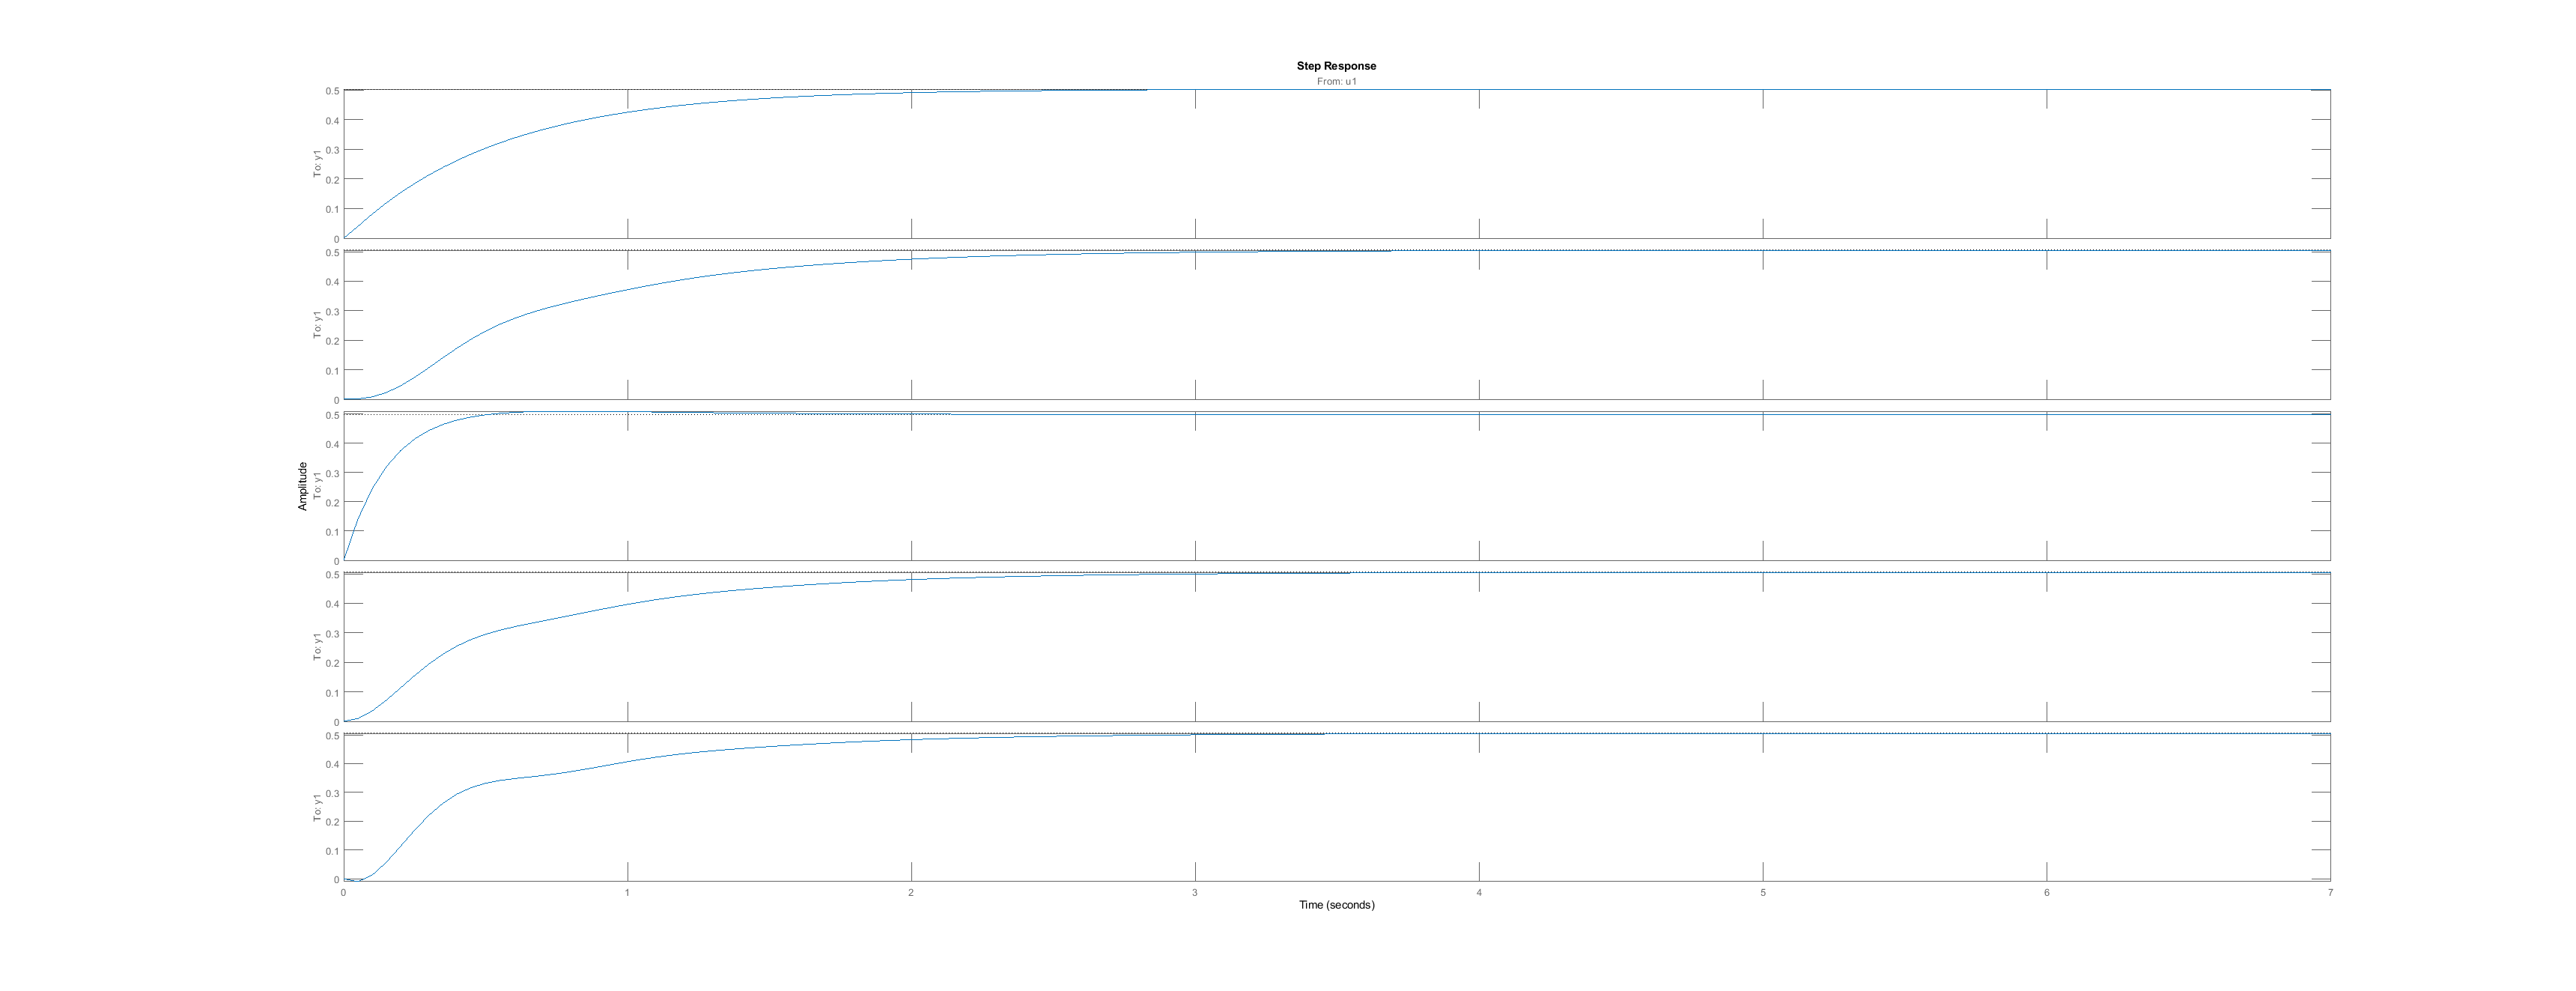
\includegraphics[width=\linewidth]{img/task_03_07__100_steps.png}
    \caption{Step responses of all the transfer functions estimated.}
    \label{fig:task 03-07 steps}
\end{figure}
\end{landscape}

\begin{figure}
    \centering
    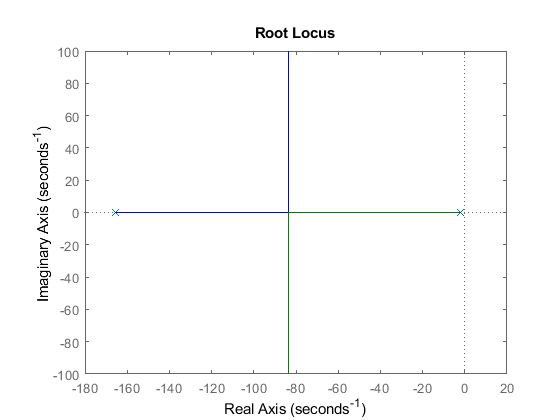
\includegraphics[width=\linewidth]{img/task03_110_rlocus.png}
    \caption{Root locus of $2^o$ transfer function with $0$ zeroes.}
    \label{fig:task rlocus 2o/0}
\end{figure}

This transfer function produces
\begin{itemize}
    \item overdamped in $\brao{0, 42.9}$
    \item critically damped at $\Brac{42.9}$
    \item underdamped in $\brao{42.9, \infty}$
\end{itemize}

\begin{figure}
    \centering
    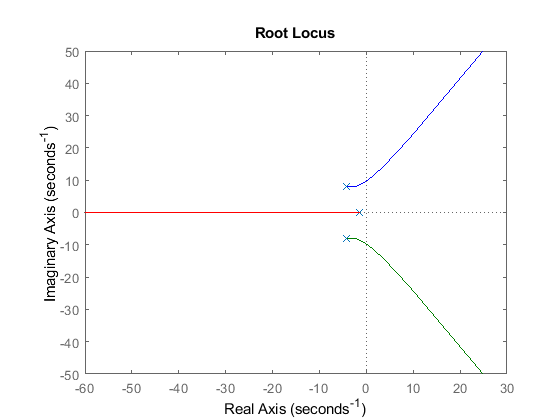
\includegraphics[width=\linewidth]{img/task04_110_rlocus.png}
    \caption{Root locus of $3^o$ transfer function with $0$ zeroes.}
    \label{fig:task rlocus 3o/0}
\end{figure}

This transfer function produces
\begin{itemize}
    \item overdamped in $\brao{0, \infty}$
    \item underdamped in $\brao{0, 13}$
\end{itemize}

\begin{figure}
    \centering
    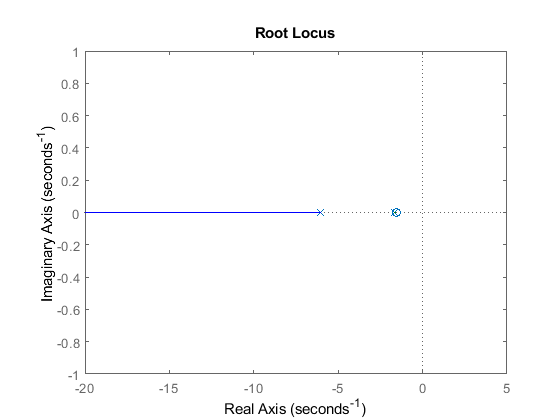
\includegraphics[width=\linewidth]{img/task05_110_rlocus.png}
    \caption{Root locus of $2^o$ transfer function with $1$ zeroes.}
    \label{fig:task rlocus 2o/1}
\end{figure}

This transfer function produces
\begin{itemize}
    \item overdamped in $\brao{0, \infty}$
\end{itemize}

\begin{figure}
    \centering
    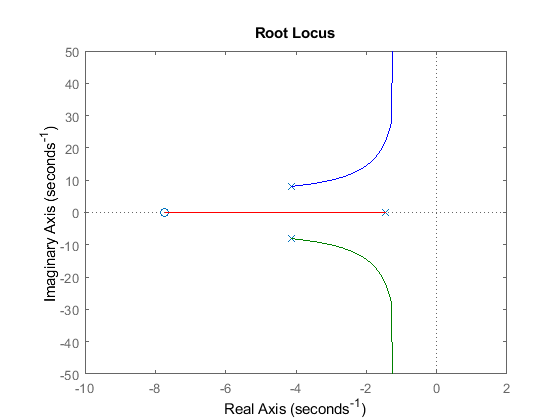
\includegraphics[width=\linewidth]{img/task06_110_rlocus.png}
    \caption{Root locus of $3^o$ transfer function with $1$ zeroes.}
    \label{fig:task rlocus 3o/1}
\end{figure}

This transfer function produces
\begin{itemize}
    \item overdamped in $\brao{0, \infty}$
    \item underdamped in $\brao{0, \infty}$
\end{itemize}

\begin{figure}
    \centering
    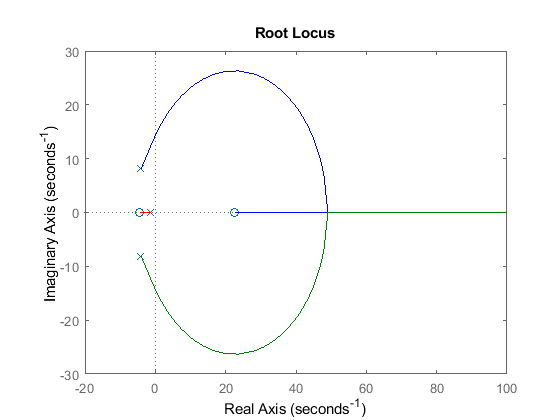
\includegraphics[width=\linewidth]{img/task07_110_rlocus.png}
    \caption{Root locus of $3^o$ transfer function with $2$ zeroes.}
    \label{fig:task rlocus 3o/2}
\end{figure}

This transfer function produces
\begin{itemize}
    \item overdamped in $\brao{0, \infty}$
    \item underdamped in $\brao{0, 10.3}$
\end{itemize}

\section{Discussion}\label{sec:Discussion}

(Note that I accidentally deleted the images used to setup the System Identification Toolkit, so I recycled the ones from the Simulink Control Design in Lab 09. I will fix this in the final version of Lab 10.)

\newpage
\printbibliography

\newpage
\appendix
\section{Appendix}\label{app}

\subsection{Task 01 -- Analyzing data and initial parameters, Matlab script}\label{sap:initial params}
\inputminted{matlab}{src/week01_task01_params.m}

\hr{}

\subsection{Task 03--07 -- Estimating transfer functions based on order, plot step responses, root locus}\label{sap:tfest}
\inputminted{matlab}{src/week01_tasks_03_07_step_rlocus.m}

\end{document}
